\section{Background}
\subsection{Word Embeddings}
A word embedding is a function mapping from words to their continuous vector representations.
The purpose of this method is to encode relevant syntactic and semantic features of words as relationships among their representation vectors.
Usually, word embeddings are trained on large, unlabeled corpus~\cite{glove,word2vec} and then fine-tuned with respect to specific NLP tasks~\cite{treeLSTM,KimCNN}.   
Pre-learned word presentations have been applied widely and become the ``secret sauce'' for the success of recent NLP systems~\cite{Luong_betterword}.
\subsubsection{Matrix presentation of sequences of words}
Suppose that \(Z = \{e_0, e_1, \ldots e_m\}\) is a set input channels with each channel uses an independent word embedding, any sentence~\(s\) of length~\(n\) can be represented as a matrix.
For indexing, the first word in a sentence is word-\(0\)th.
In case the sentence is padded with dummy words on its left, these padded dummy words are indexed by negative integers.

For any word embedding~\(e\), the vector presentation of the word-\(i\)th is denoted as~\(w^{(e)}_i \in \mathbb{R}^{d_e}\).
The vector presentation of word-\(i\)th through the set of input channels \(Z\) can be expressed as follow:
\begin{align}
 x_i &= w^{(e_0)}_i \ominus w^{(e_1)}_i \ominus  \ldots \ominus w^{(e_m)}_i&\label{concat-emb}
\end{align}
In Eq.\eqref{concat-emb}, \(\ominus\) is concatenation operator which result in the vector \(x_i \in \mathbb{R}^{d}\) with \(d = \sum_{e \in Z} d_e\).
Any sequence of words in the sentence which start at word-\(i\)th and end at word-\(j\)th can be presented as the following matrix:
\begin{align}
X_{i:j} &= x_i \oplus x_{i+1} \oplus \ldots \oplus x_j &\label{concat}
\end{align}
In Eq.\eqref{concat}, \(\oplus\) is concatenation operator which result in the matrix \(X_{i:j} \in \mathbb{R}^{d \times (j-i+1)}\).
\subsection{Convolution and Pooling}
Convolution Neural Networks (CNNs) have been proven to be effective models for the task of sentence-level sentiment analysis~\cite{KimCNN, DCNN,2-layer-cnn}.
Convolution Neural Networks are commonly constructed by staking up multiple convolution, pooling and fully connected layers.
\subsubsection{Convolution Layer}\label{conv-layer}
Given that \(F\) is the set of all filters of the convolution layer, for any filter \(v \in F\) which has window size \(l\) and set of parameters \(\theta^{(v)} = \{ W^{(v)}, b^{(v)} | W^{(v)} \in \mathbb{R}^{d \times l}, b^{(v)} \in \mathbb{R}\}\), filter \({v}\) is applied on any sequence of word-\(i\)th to word-\((i+l-1)\)th through the following equation:
\begin{align}
c^{(v)}_j &= f(W^{(v)} \otimes X_{i:i+l-1} + b^{(v)}) &\label{filter}
\end{align}
In Eq.\eqref{filter}, operator \(\otimes\) is the Hadamard product~\cite{element-prod}.  
\(b \in \mathbb{R}\) as bias term and \(f\) is an activation function.
For indexing, \(j = i + x\) with \(x \in \mathbb{N}\) and \(0 \leq x < l\).
If half-padding policy is employed then \(j = i + \floor{\frac{l}{2}}\).

By slicing the filter \(v\) through the sentence (i.e. applying the filter \(v\) on different sequences of length \(l\) along the sentence) we can get vector \(c^{(v)} = [c^{(v)}_0, c^{(v)}_1~\cdots]\) which is a feature map of the sentence~\(s\).
The length of the feature map \(c^{(v)}\) depends on the length of the input sentence.
Additionally, the length of \(c^{(v)}\) also depends on the way filter \(v\) was slided through the sentence and its window size \(l\)~\cite{conv-arith}.
In summary, each filter produces a variable-length feature map of the sentence.
As a result, when applying a convolution layer on a sentence, we get a set of variable-length feature maps.
\subsubsection{Max Pooling Layer}
For dealing with the problem of variable-length feature maps, several types of max pooling layer was employed.
In general, given a input vector \(i\), a \(k\)-max pooling layer reduces the size of vector \(i\) by extracting the largest \(k\) entries from \(i\).
In case \(k = 1\) the pooling layer is called max-over-time pooling~\cite{nlp-scratch,KimCNN}.
Apart from being treated as a hyper-parameter, \(k\) can also be parameterized with respect to the length of the input sentence, in which case, the pooling layer is called dynamic k-max pooling~\cite{DCNN}.
\subsection{Recurrent Neural Network}
By definition, Recurrent Neural Networks are any Neural Networks which have at least a recurrent connection~\cite{rnn-def}.
Recurrent Neural Networks have been proven to be effective network architects when applying on the type of problems whose output is determined by a variable-length input sequence~\cite{speech-lstm,SutskeverVL14,mikolov-nlm}.
\subsubsection{Vanilla Recurrent unit}\label{sec:vanilla-rnn}
Denoting input sequence as \(I = \{i_0,\ldots,i_n\}, \forall t, i_t \in \mathbb{R}^n\), Vanilla Recurrent unit can be expressed as the following recursive formula~\cite{treeLSTM}:
\begin{align}
h_t &= tanh(Wi_t + Uh_{t-1} + b)&
\end{align}
For sentence-level sentiment analysis, \(h_n\) is treated as output of the network.
In theory, Vanilla Recurrent Neural Network is Turing-Complete~\cite{rnn-turing-complete} but hard to train (especially on long input sequence) due to the problems of exploding and vanishing gradient~\cite{Bengio1994}.
To mitigate the problem of vanishing gradient, Long Short Term Memory unit (LSTM)~\cite{originLSTM} unit was invented.
\subsubsection{Long Short Term Memory unit}\label{sec:lstm}
Long Short Term Memory unit can be expressed as the following recursive formula~\cite{treeLSTM}:
\begin{align}
w_t &= \sigma(W^{(w)}i_t + U^{(w)}h_{t-1} + b^{(w)}) \label{eq:lstm-input-gate}&\\
f_t &= \sigma(W^{(f)}i_t + U^{(f)}h_{t-1} + b^{(f)}) \label{eq:lstm-forget-gate}&\\
o_t &= \sigma(W^{(o)}i_t + U^{(o)}h_{t-1} + b^{(o)}) \label{eq:lstm-output-gate}&\\
u_t &= tanh(W^{(u)}i_t + U^{(u)}h_{t-1} + b^{(u)}) \label{eq:lstm-update-gate}&\\
c_t &= r_t \otimes u_t + f_t \otimes c_{t-1} \label{eq:longterm-mem}&\\
h_t &= o_t \otimes tanh(c_t) \label{eq:temperal-mem}&
\end{align}
Traditionally, \(w_t\), \(f_t\) and \(o_t\) are called input/write gate, forget/deallocate gate and output/read gate respectively and \(c_t\) is called memory cell.
Intuitively, we can interpret how the network works as follow: 
in the above formula, \(h_{t-1}\) can be viewed as a short-term memory of the network; 
\(u_t\) is the information extracted from in current input \(i_t\) and the short-term memory \(h_{t-1}\); 
write gate \(w_t\) decides which information from \(u_t\) will be written into the memory cell \(c_t\); 
forgot gate \(f_t\) decides which information while be preserved on memory cell \(c_t\); 
and \(o_t\) decides which information will be read from the memory cell \(c_t\), which will produce the short-term memory (or output) \(h_t\).
\subsection{Recursive Neural Network}
In most cases, to understand a sentence, we must understand the phrases composing it, in turn, to understand a phrase, we must understand the phrases and words composing the phrase.
Recursive Neural Networks were mainly inspired by this idea~\cite{treeLSTM}.
Given a sentence and its parse tree, a Recursive Neural Network composes the vector presentation of the sentence by applying it composition function at each node of the parse tree in a bottom-up manner.
For demonstration, parse tree of the phrase ``is very interesting'' and its composing process using a Recursive Neural Network are illustrated in Fig.\ref{fig:example-parse} and Fig.\ref{fig:example-compose} respectively~\cite{tag-embedding-rnn}.
\begin{figure}[] 
	\centering
	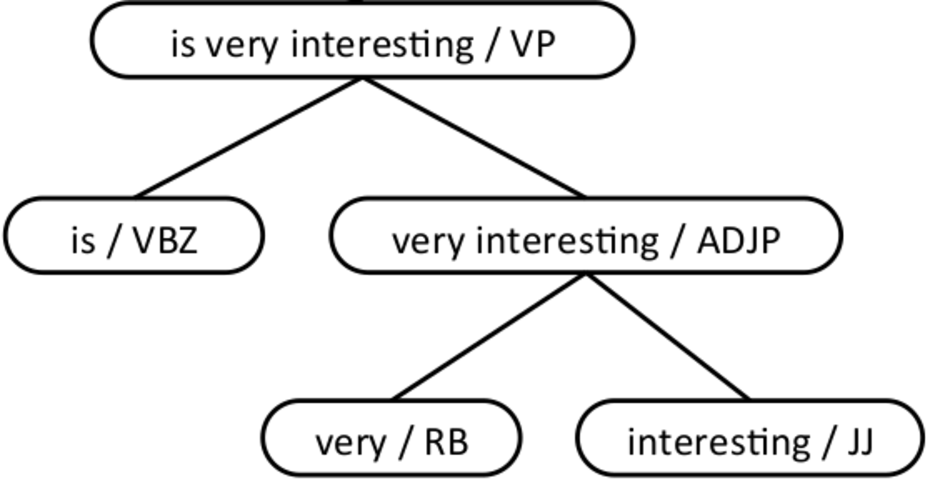
\includegraphics[scale=0.4]{figure/example-parse}
	\caption[Constituency parse tree for the phrase ``is very interesting'']{Constituency parse tree for the phrase ``is very interesting''.}
	\label{fig:example-parse}
\end{figure}
\begin{figure}[]
	\centering
	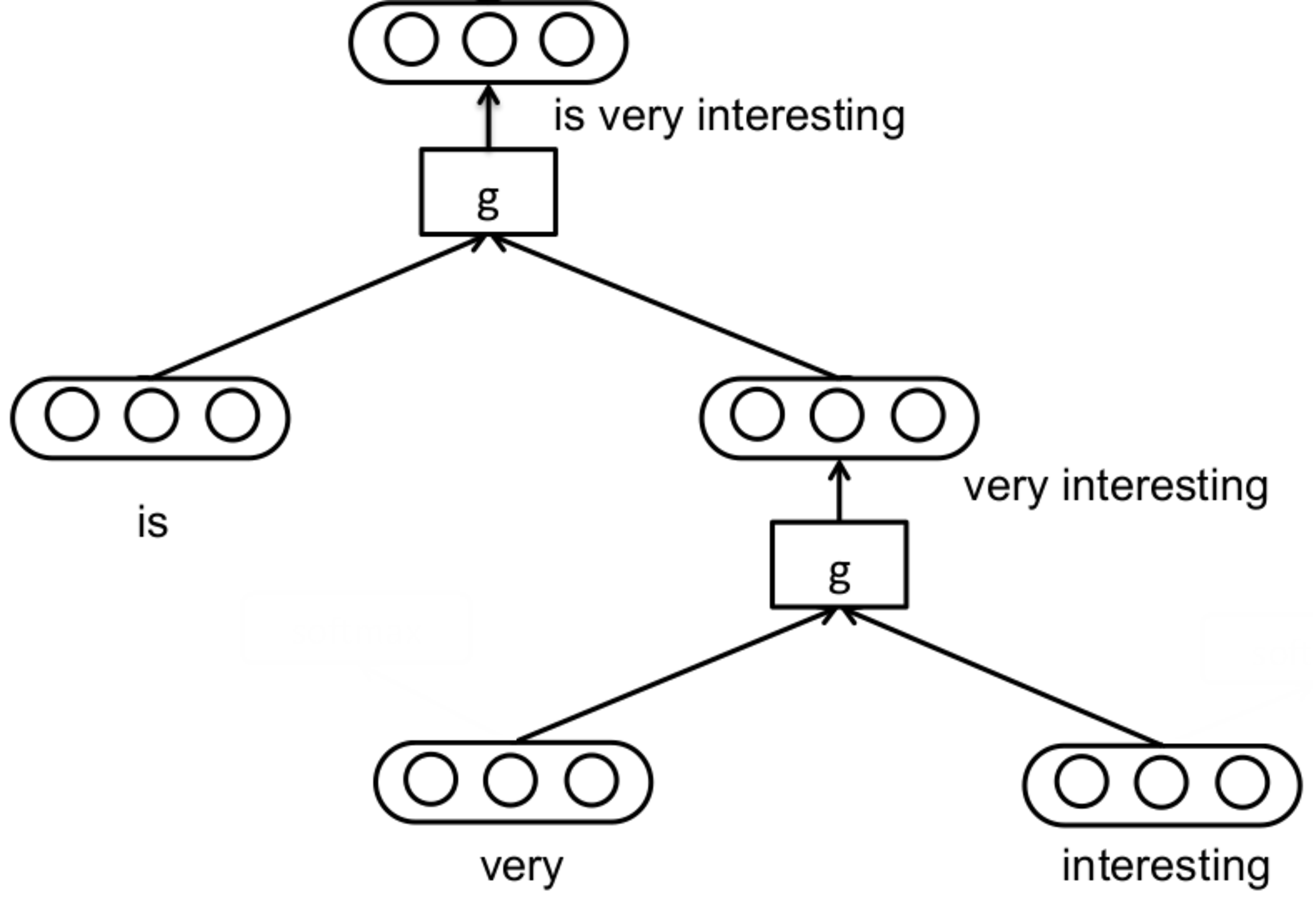
\includegraphics[scale=0.3]{figure/example-compose}
	\caption[Applying Recursive Neural Network on the phrase ``is very interesting'']{Applying Recursive Neural Network on the Constituency parse tree of the phrase ``is very interesting''.
		The composition function of this network is denoted as \textbf{g}.}
	\label{fig:example-compose}
\end{figure}

One of the most successful Recursive Neural Networks are Tree-LSTMs~\cite{treeLSTM}.
The core idea behind the design of Tree-LSTMs are to generalize the LSTM for tree-structured inputs.
Tree-LSTMs were able to archive state-of-the-art performance on two tasks: predicting the semantic relatedness of two sentences (SemEval 2014, Task 1~\cite{SemeEvalTask1}) and sentiment classification (Stanford Sentiment Treebank~\cite{socher2013recursive}).
\subsubsection{Constituency Tree-LSTM}\label{treelstm}
Let \(d\) be the size of the input vectors, \(r
\) be the size of the memory cell and \(z\) be the number of sentiment classes. 
\paragraph{Leaf module}
Given any input vector \(x \in \mathbb{R}^d\), the calculation steps inside the leaf module can be expressed as follow:
\begin{align}
o &= \sigma{\left( W^{(o)} x + a^{\left(o\right)}\right)} & \\
c &= W^{(c)} x + a^{(c)} & \\
h &= o \odot \tanh{\left(c\right)} &
\end{align}
In this module, \(W^{(o)}, W^{(c)} \in \mathbb{R}^{r \times d}\) and \(a^{\left(o\right)}, a^{(c)} \in \mathbb{R}^r\).
\paragraph{Composer module}
Given the input vectors \({h_l}\), \({c_l}\) from the left child node and \({h_r}\), \({c_r}\) from the right child node, the calculation steps inside the composer module can be expressed as follow:
\begin{align}
i &= \sigma{ \left(U_l^{(i)} h_{l} + U_r^{(i)} h_{r} + b^{(i)} \right) } &\\
f_{l} &= \sigma{\left(U_{l}^{(l)} h_{l} + U_{r}^{(l)} h_{r} + b^{(f)}\right)} & \\
f_{r} &= \sigma{\left(U_{l}^{(r)} h_{l} + U_{r}^{(r)} h_{r} + b^{(f)}\right)} & \\
o &= \sigma{\left( U_l^{(o)} h_{l} + U_r^{(o)} h_{r} + b^{(o)}\right)} &\\
u &= \tanh{\left( U_l^{(u)} h_{l} + U_r^{(u)} h_{r} + b^{(u)}\right)} &\\
c &= i \odot u + f_{l} \odot c_{l} + f_{r} \odot c_{r} & \\
h &= o \odot \tanh{\left(c\right)} &
\end{align}
In this module, for any \(j \in \{i, l, r, o, u\}\) and \(x \in \{\l, r\}\), \(U_x^{(j)} \in \mathbb{R}^{r \times r}\) and \( b^{(j)} \in \mathbb{R}^r\).
\paragraph{Output module}
Denoting sequence of words spanned by a sub-tree rooted at node \({j}\) as \({\{x\}_j}\).
Given \({h_j}\) is the \({h}\) output of node \({j}\), the prediction at node \({j}\) can be computed by the output module as follow:
\begin{align}
\hat{p_{\theta}}(y \mid \{x\}_j ) &= softmax( W^{(s)} h_j + b^{(s)}) & \\
\hat{y_j} &= \underset{y}{\mathrm{argmax}} \; \hat{p_{\theta}}(y \mid \{x\}_j ) &
\end{align}
In this module, \(W^{(s)} \in \mathbb{R}^{z \times r}\) and \( b^{(s)} \in \mathbb{R}^z\).
\paragraph{Composing sentence}
Given any sentence, its parse tree and a word embedding, each word in the sentence is mapped to a representation vector.
For any non-leaf node, composer module is applied recursively and for any leaf node, the leaf module is applied on the vector representation of the corresponding word.
Finally, we can apply the output module on any node in the parse tree.
Recursive Neural Networks have several advantages over Recurrent Neural Networks: 
\begin{itemize}
	\item In case the input sequence belongs to a recursively defined language, given only a small subset of the data with limited length sentences, tree structures model have better ability to generalize comparing to sequential ones.
	However, when the limited length of sentences in the training data is increased, the advantage of tree over sequential models decrease fast~\cite{bowman-treevslstm}. 
	\item Tree can breaks down complicated sentences into simpler phrases, which make it easier for generalization~\cite{knowledge-matter}~\cite{need-tree}.
	\item Some features which are far apart when a sentence is presented as sequence become closer when it is presented as tree~\cite{need-tree}.
\end{itemize}